\documentclass[../lab2.tex]{subfiles}

\begin{document}

    In questo primo caso utilizziamo una virtual machine Linux e un pc con una Live
    USB Linux collegato al primo tramite un router.
    Abbiamo effettuato l'accesso remoto dal primo al secondo host tramite il comando SSH. 
    Per la connessione si e' utilizzato un cavo ethernet (cat 5e).
    Abbiamo settato dal PC Live Linux tramite il comando "sudo ethtool -s eth0 speed 
    10 duplex full autoneg on" la velocita' di trasmissione con lo switch a 10 Mb/s.
    Mentre non si puo' stabilire la reale velocita' che abbiamo tra virtual switch
    e porta ethernet della virtual machine e USB, come si puo' notare dalla
    figura che rappresenta la configurazione.

    \begin{center}
        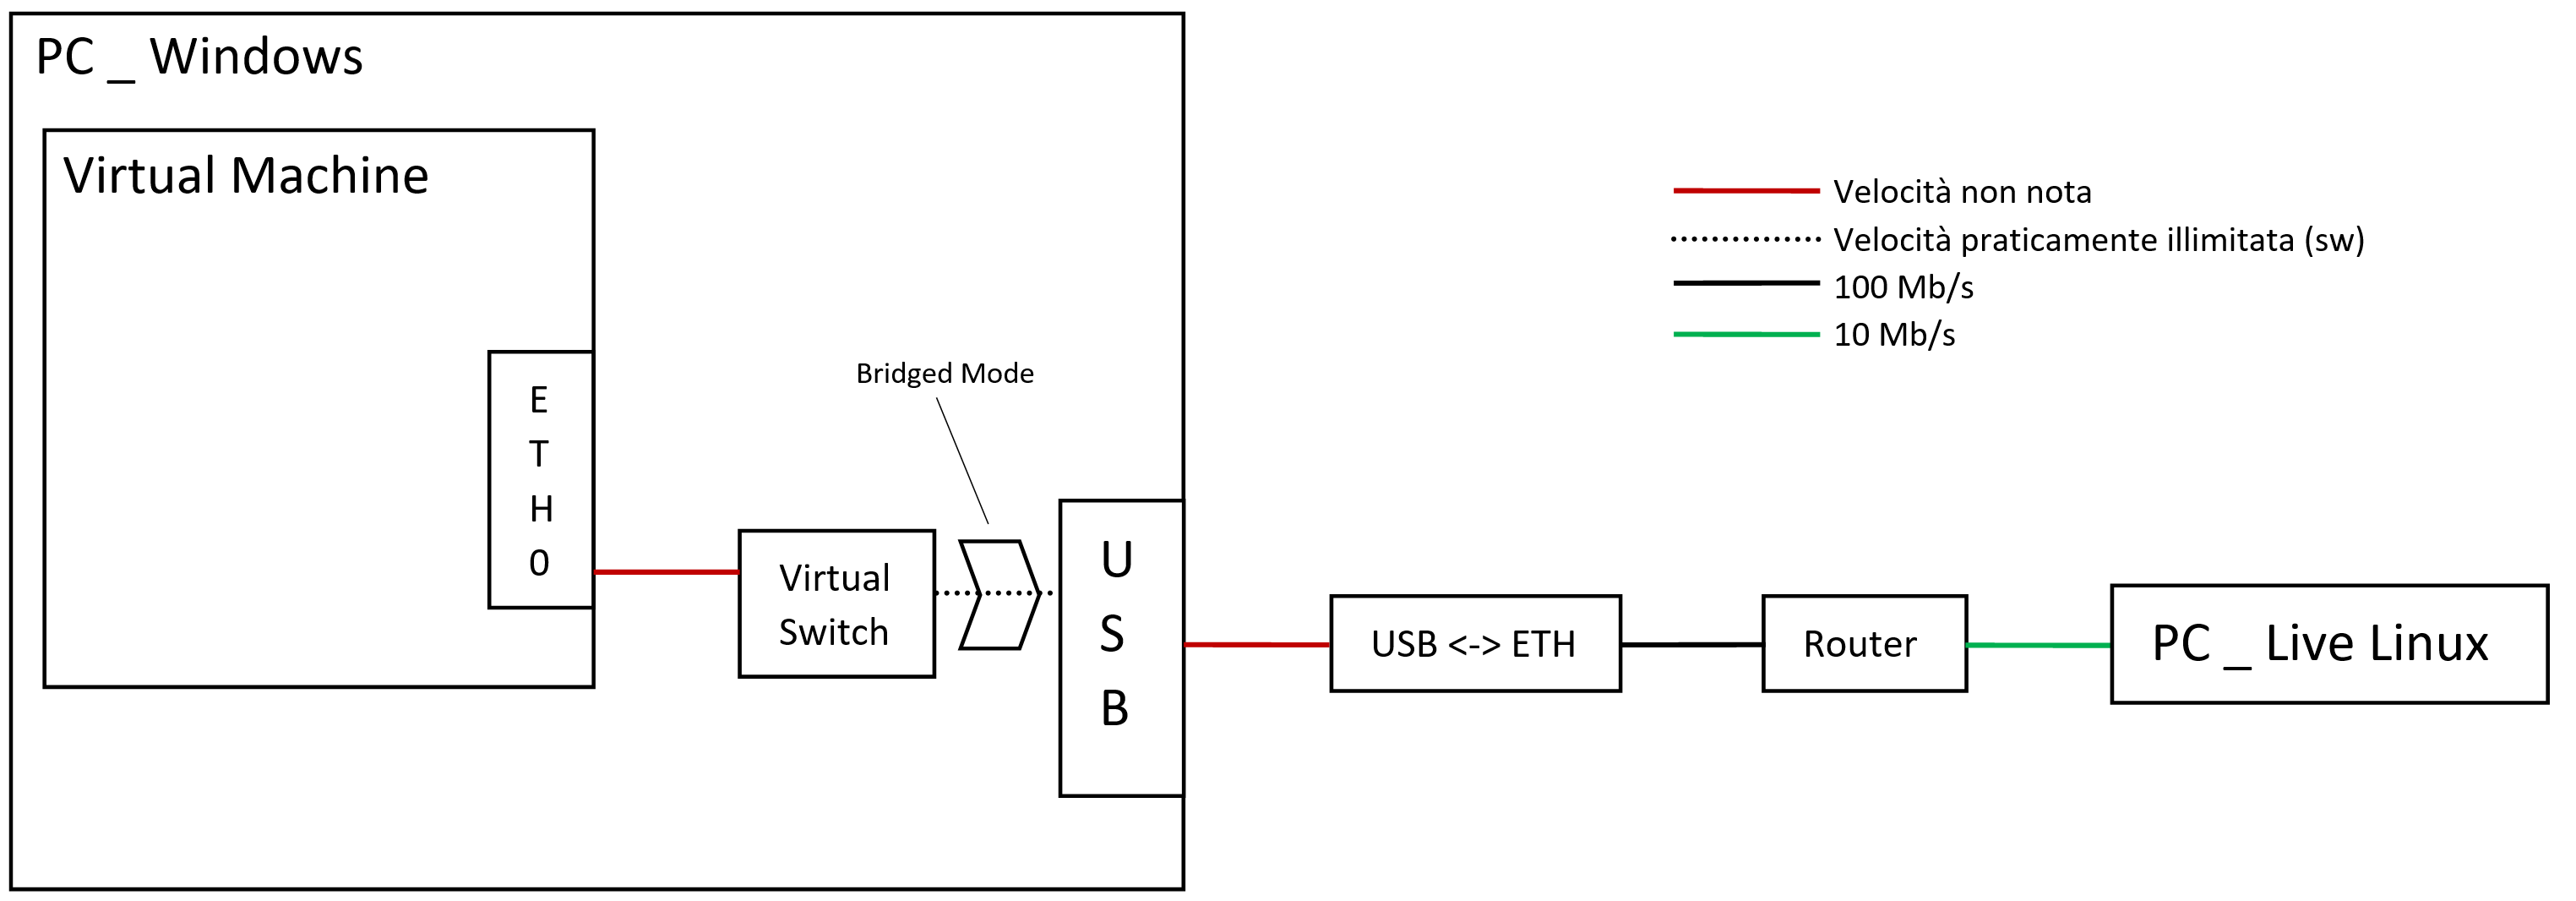
\includegraphics[scale=0.14]{Config1.png}
    \end{center}

\end{document}